% Standalone TikZ source for the conceptual mixed-layer step-change figure.
% GitHub Markdown does not render TikZ directly; the SVG version is embedded
% in dynamic-mixed-layer-depth.md. This source is retained for papers/slides.
\documentclass[tikz,border=8pt]{standalone}
\usepackage{amsmath}
\usetikzlibrary{arrows.meta,decorations.pathmorphing,positioning}
\begin{document}
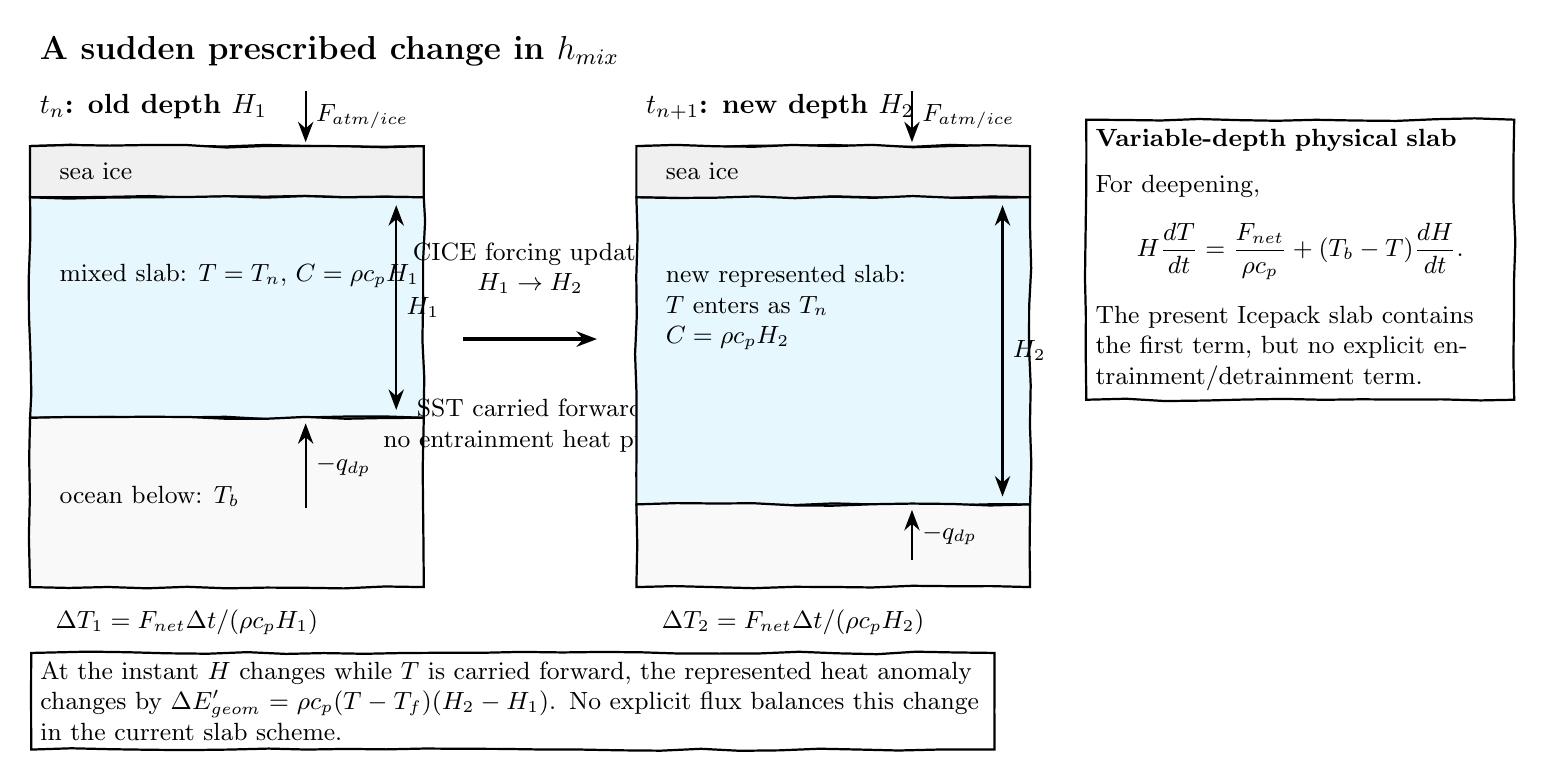
\begin{tikzpicture}[
  font=\small,
  >={Stealth[length=2.6mm]},
  rough/.style={draw,thick,decorate,decoration={random steps,segment length=5mm,amplitude=.5pt}},
  flux/.style={->,thick},
  note/.style={align=left,text width=4.0cm}
]
\node[font=\bfseries\large,anchor=west] at (0,8.2)
  {A sudden prescribed change in $h_{mix}$};

% t_n
\node[font=\bfseries,anchor=west] at (0,7.5) {$t_n$: old depth $H_1$};
\draw[rough] (0,7) -- (5,7);
\filldraw[fill=gray!12,rough] (0,7) rectangle (5,6.35);
\node[anchor=west] at (.25,6.68) {sea ice};
\filldraw[fill=cyan!10,rough] (0,6.35) rectangle (5,3.55);
\node[anchor=west] at (.25,5.35) {mixed slab: $T=T_n$, $C=\rho c_p H_1$};
\filldraw[fill=gray!5,rough] (0,3.55) rectangle (5,1.4);
\node[anchor=west] at (.25,2.55) {ocean below: $T_b$};
\draw[flux] (3.5,7.7) -- (3.5,7.05) node[midway,right] {$F_{atm/ice}$};
\draw[flux] (3.5,2.4) -- (3.5,3.48) node[midway,right] {$-q_{dp}$};
\draw[<->,thick] (4.65,6.25) -- (4.65,3.65) node[midway,right] {$H_1$};
\node[anchor=west] at (.2,.95) {$\Delta T_1=F_{net}\Delta t/(\rho c_p H_1)$};

% update
\draw[->,very thick] (5.5,4.55) -- (7.2,4.55);
\node[align=center] at (6.35,5.45) {CICE forcing update\\$H_1\rightarrow H_2$};
\node[align=center] at (6.35,3.45) {SST carried forward\\no entrainment heat pulse};

% t_n+1
\node[font=\bfseries,anchor=west] at (7.7,7.5) {$t_{n+1}$: new depth $H_2$};
\draw[rough] (7.7,7) -- (12.7,7);
\filldraw[fill=gray!12,rough] (7.7,7) rectangle (12.7,6.35);
\node[anchor=west] at (7.95,6.68) {sea ice};
\filldraw[fill=cyan!10,rough] (7.7,6.35) rectangle (12.7,2.45);
\node[note,anchor=west] at (7.95,4.95) {new represented slab:\\$T$ enters as $T_n$\\$C=\rho c_pH_2$};
\filldraw[fill=gray!5,rough] (7.7,2.45) rectangle (12.7,1.4);
\draw[flux] (11.2,7.7) -- (11.2,7.05) node[midway,right] {$F_{atm/ice}$};
\draw[flux] (11.2,1.75) -- (11.2,2.38) node[midway,right] {$-q_{dp}$};
\draw[<->,thick] (12.35,6.25) -- (12.35,2.55) node[midway,right] {$H_2$};
\node[anchor=west] at (7.9,.95) {$\Delta T_2=F_{net}\Delta t/(\rho c_p H_2)$};

% Missing physics
\node[draw,rough,align=left,text width=5.2cm,anchor=north west] at (13.4,7.35) {
\textbf{Variable-depth physical slab}\\[2mm]
For deepening,
\[
H\frac{dT}{dt}=\frac{F_{net}}{\rho c_p}+(T_b-T)\frac{dH}{dt}.
\]
The present Icepack slab contains the first term, but no explicit entrainment/detrainment term.};

\node[draw,rough,align=left,text width=12cm,anchor=west] at (0,-.05) {
At the instant $H$ changes while $T$ is carried forward, the represented heat anomaly changes by
$\Delta E'_{geom}=\rho c_p(T-T_f)(H_2-H_1)$. No explicit flux balances this change in the current slab scheme.};
\end{tikzpicture}
\end{document}
